\documentclass[11pt]{article}
\usepackage[a4paper,left=25mm,right=25mm,top=22mm,bottom=22mm]{geometry}
\usepackage{amsmath,amssymb,amsthm,booktabs,xcolor,fancyhdr,graphicx,tikz}
\usepackage[hidelinks]{hyperref}
\definecolor{ink}{RGB}{31,65,87}
\newtheoremstyle{noteplain}{6pt}{4pt}{\itshape}{}{\bfseries\color{ink}}{.}{0.55em}{}
\theoremstyle{noteplain}
\newtheorem{lemma}{Lemma}
\newtheorem{theorem}{Theorem}
\newtheorem{proposition}{Proposition}
\newcommand{\norm}[1]{\lVert #1\rVert}
\newcommand{\ip}[2]{\langle #1,#2\rangle}
\newcommand{\dates}[2]{\{#1,\ldots,#2\}}
\newcommand{\dd}{\dagger}
\setlength{\parindent}{0pt}
\setlength{\parskip}{4pt plus 1pt}
\setlength{\emergencystretch}{2em}
\setlength{\headheight}{14pt}
\pagestyle{fancy}\fancyhf{}
\lhead{\small MATH 4999}\rhead{\small First threshold crossing}
\rfoot{\small\thepage}\renewcommand{\headrulewidth}{0.25pt}
\begin{document}
{\Large\bfseries\color{ink} Numerical Stability and Error Propagation in\\[2pt] Autoregressive World-Model Rollouts}\par
{\large\color{ink} First-Threshold-Crossing Bounds and Source-Level Calibration}\par
{\small Capstone research draft \hfill 10 November 2026}

\begin{abstract}
A video rollout may exceed an error tolerance within a control chunk even when its chunk endpoints appear acceptable. This report studies the first future frame whose RGB root-mean-square error strictly exceeds a fixed threshold. We derive deterministic exclusions from radial and angular information and invert a total motion-energy constraint: a crossing is feasible at an attained minimum when the reference is already outside the safe ball, but requires strictly positive surplus otherwise. A scalar-error majorant is sharp in an unrestricted product Hilbert space. Pixel constraints additionally yield two-sided calibration bounds and nested candidate sets. A retrospective box-bound diagnostic lowered the calibrated upper threshold by about $20.52\%$ without narrowing the observed test set. Source-level calibration gives a conditional $5/6$ marginal guarantee for both schedules when calibration and new-source scores are exchangeable given development data. A retrospective replay uses 16 sources, split 5/5/6 into development, calibration and test; all 32 scalar error traces and all real RGB videos are available. Generated 48-frame prefixes are available for three sources, including only one of the 12 test schedules. The event-score calibration threshold is $52.9\%$ smaller than the total-motion-energy calibration threshold but leaves 80 of 81 labels in that test schedule, while the 11 other test schedules use universal fallback. The scalar-information floor analysis certifies that lowering the threshold alone cannot remove frame 21 in that test prefix; the later box diagnostic retains the zero lower certificate and gives the native threshold an outward enclosure $[0,33.818]$. The replay therefore does not establish a useful narrower individual prediction set. Previously examined sources and missing generated vectors limit prospective interpretation.
\end{abstract}

\section{Introduction}\label{sec:intro}
This study is motivated by error propagation over rollout horizons. Here we focus on when frame-level error first exceeds a tolerance, while local amplification and low-dimensional error structure remain separate questions.

The time at which a generated video first departs from its reference beyond a chosen tolerance is a useful frame-level description of rollout error. A terminal or chunk-level bound alone need not determine this event: errors can cross the threshold and later return. This report asks which crossing times can be excluded using motion information, and what can be said when that information is calibrated from separate source videos.

The report makes three contributions. First, it derives deterministic frame-error bounds and an exact inversion of a total-energy region, including the strict boundary of the crossing event. Second, it constructs a sharp scalar-error majorant and gives source-level rank guarantees under explicit exchangeability assumptions. Third, it compares these constructions in a retrospective replay and reports where the available information fails to produce a useful narrowing. The conformal rank framework is established background \cite{vovk2005,diquigiovanni2021}; the event-specific derivations and their scope are stated below. The data have been examined previously, so the replay is diagnostic rather than a prospective validation.

\section{Problem and available information}\label{sec:problem}
The study contains 16 source videos, each with two native rollout schedules. All 32 scalar error traces and the real RGB videos for all 16 sources are available. Generated RGB prefixes of 48 frames are locally available for three sources, of which one is a test source; thus only one of 12 test schedules has a generated prefix for direct pixel-based evaluation. The source split is five development (DEV), five calibration (CAL), and six test (TEST) sources. Coverage of a source means inclusion of both schedule labels. The generated model is fixed, and the recorded control schedules used observed future poses offline. At the operational prediction point the generated rollout or prefix is already available, but future true RGB frames have not been used for evaluation. Deployment requires the relevant control inputs to be available. This task does not predict $T$ before generation or establish model dynamics or fine-tuning fairness.

In the 29 September 2026 notes, \emph{Mathematical Foundations for Finite-Horizon Error and Response Analysis}, $e=\widehat x-x$ denoted prediction minus reference, with one time step per action chunk. Here $t$ counts individual future RGB frames. The distinction matters: two rollouts can agree at the end of a chunk and have different errors inside it. We therefore work directly with frame errors and take the forecast as given.

Let $x_0$ be the observed initial frame, $x_t$ the real frame, and $\widehat x_t$ the generated frame, all in $[0,1]^D$, with $D=3\cdot256^2$. Write
\[
 \ip{u}{v}=D^{-1}\sum_{i=1}^D u_i v_i,\qquad
 \norm{u}=\sqrt{\ip{u}{u}},\qquad E_t=\norm{\widehat x_t-x_t}.
\]
With $H=80$ and $\tau$ the stored binary64 value of $0.20$, define
\[
 T=\min\{1\le t\le H:E_t>\tau\},
 \qquad T=\dd\quad\text{if the set is empty}.
\]
The symbol $\dd$ records that the rollout stayed within tolerance for all 80 frames. A tie at the threshold counts as safe.

\textbf{What would connect the old bound to this target?}
Let $B$ bound the error in a chunk's input state, $\norm{\widehat z-z}_{\rm state}\le B$. Let $G_j$ output the $j$th RGB frame of that chunk under the same controls and seed, with $\widehat x_t=G_j(\widehat z)$. If $G_j$ is $K_j$-Lipschitz from the state norm to RGB RMS on these inputs, adding and subtracting $G_j(z)$ gives
\[
 E_t\le K_j B+\norm{G_j(z)-x_t}.
\]
This would require a within-chunk response bound and a reference-input frame defect. The frame-level argument below instead uses measured RGB quantities.

\section{Deterministic bounds}\label{sec:deterministic}
The following exclusions are conditional on the stated bounds. They identify necessary conditions on a crossing time and do not assume that error is monotone.

\begin{lemma}[First-crossing exclusion]\label{lem:exclude}
Assume $L_t\le E_t\le U_t$ simultaneously for the trajectory under consideration. Then every possible finite $T$ belongs to
\[
 \mathcal A_{\rm fin}=\{t\in\dates{1}{H}:U_t>\tau,\ L_s\le\tau\ \text{for all }s<t\}.
\]
Include $\dd$ in the outer set exactly when $L_s\le\tau$ for every $s\le H$.
\end{lemma}
\begin{proof}
If $T=t$, then $E_t>\tau$, so $U_t>\tau$. Every earlier $E_s$ was at most $\tau$, hence $L_s\le\tau$. If $T=\dd$, the same inequality holds for every frame. These cases exhaust the outcomes.
\end{proof}

\textbf{When does this give an exact frame?} If $U_s\le\tau$ for every $s<k$ and $L_k>\tau$, then $T=k$. Knowing only $L_k>\tau$ establishes $T\le k$; the rollout might have crossed earlier and returned. No monotonicity is needed. When different times are coupled, a date that survives the lemma may still lack a feasible whole-video trajectory.

\subsection{Radial and directional information}
Use the same origin $r=x_0$ for both paths. Set $g_t=\widehat x_t-r$, $v_t=x_t-r$, $d_t=\norm{g_t}$ and $b_t=\norm{v_t}$. These motions are changes in RGB pixel values. For $d_tb_t>0$ put $c_t=\ip{g_t}{v_t}/(d_tb_t)$. Expanding a squared norm gives
\begin{equation}
 E_t^2=\norm{g_t-v_t}^2=d_t^2+b_t^2-2d_tb_tc_t . \label{eq:geometry}
\end{equation}
When $d_tb_t=0$ the cross term vanishes. Distance from the first frame alone therefore misses a quantity directly relevant to error: the alignment of real and generated changes.

\begin{theorem}[Bounds from radial and angular intervals]\label{thm:geometry}
At a fixed frame suppose $d=d_t$ is known, $0\le\ell\le b_t\le h$, and $c_-\le c_t\le c_+$ whenever $db_t>0$, where $-1\le c_-\le c_+\le1$. Write $\bar b=\min(h,\max(\ell,dc_+))$. Then
\begin{align}
 E_t^2 &\ge (\bar b-dc_+)^2+d^2(1-c_+^2), \label{eq:min}\\
 E_t^2 &\le \max_{\beta\in\{\ell,h\}}\{d^2+\beta^2-2d\beta c_-\}. \label{eq:max}
\end{align}
These are the exact extrema of the scalar expression over the stated rectangle in length and cosine.
\end{theorem}
\begin{proof}
For each $\beta\ge0$, $d^2+\beta^2-2d\beta c$ decreases weakly as $c$ increases. For the minimum set $c=c_+$ and complete the square. The minimum squared distance from $dc_+$ to $[\ell,h]$ occurs at its nearest point $\bar b$. For the maximum set $c=c_-$. The resulting quadratic is convex in $\beta$, so it attains a maximum at one of the two endpoints. When $d=0$ or $b_t=0$, any allowed cosine gives the same cross term, zero. Equation~\eqref{eq:geometry} therefore also lies between the stated extrema in these cases.
\end{proof}

\textbf{Where does the radial interval come from?} If the radial constraints are $m_t\le b_t\le M_t$ and the adjacent real changes satisfy $\norm{x_j-x_{j-1}}\le s_j$, telescoping the changes and applying the triangle inequality gives
\[
  \ell_t=m_t,\qquad h_t=\min\Bigl(M_t,\sum_{j=1}^t s_j\Bigr).
\]
An empty interval signals incompatible premises. Bounding the cosine by $[-1,1]$ recovers the direction-free upper bound $d+h$. A narrower cosine interval can improve both sides. Only scalar extrema have been proved here: pixel limits and the requirement of a single trajectory across frames can impose further constraints.

\section{Source-level calibration and event scores}\label{sec:calibration}
Calibration operates at the source level: the two schedules of one source may be dependent. The following rank guarantee is marginal over the calibration sources and the new source, conditional on DEV; it does not condition on a realized calibration set.

\begin{proposition}[Coverage of the common rule]
Fix the development rule before drawing five calibration sources and a new source. If their six source-level scores are exchangeable, accepting scores up to the largest calibration score covers the new source with probability at least $5/6$.
\end{proposition}
\begin{proof}
For a source take the larger of its two true-label scores. Missing either label means the new source is the unique strict maximum among six scores. At most one index can be that maximum. Exchangeability makes its probability at most $1/6$ for the new index. The same argument applies to lexicographically ordered score pairs, including ties; Appendix~\ref{app:details} gives the conditional rank proof.
\end{proof}
\subsection{Motion regions and energy inversion}
The following constructions use source-level calibration and a rank argument. The separate frame-6 transfer query in Section~\ref{sec:replay} requires an additional empirical condition. Let $v_{it}=x_{it}-x_{i0}$ and fix the following quantities from the five DEV sources only,
\[
 \mu_t=\tfrac15\sum_{i\in{\rm DEV}}v_{it},\qquad
 \sigma_t=\max\left(\tfrac1{255},
  \tfrac54\sqrt{\tfrac15\sum_{i\in{\rm DEV}}\norm{v_{it}-\mu_t}^2}\right).
\]
The displayed formulas specify the intended DEV construction. In the experiment the resulting stored binary64 values of $\mu_t$ and $\sigma_t$ are fixed constants, rather than the exact real values of these formulas. The proofs allow any DEV-measurable centers and positive scales; no population-estimation guarantee is asserted for $\sigma_t$. The positive floor prevents division by zero. These are a common reference motion and a time-dependent scale. The same true motion belongs to both schedules of a source.

\begin{proposition}[A motion set valid for every query]\label{prop:tube}
For each CAL source set $S_i=\max_{t\le H}\norm{v_{it}-\mu_t}^2/\sigma_t^2$, and $B=\max_{i\in{\rm CAL}}S_i$. Under exchangeability with the next source, conditional on DEV, the event
$\norm{v_{*t}-\mu_t}\le\sigma_t\sqrt B$ for every $t$ has probability at least $5/6$. On this event, for \emph{every} forecast $g_t$,
\[
 (\norm{g_t-\mu_t}-\sigma_t\sqrt B)_+
 \le E_t\le \norm{g_t-\mu_t}+\sigma_t\sqrt B .
\]
\end{proposition}
\begin{proof}
The event is $S_*\le\max_i S_i$, so the unique-maximum proof in Section~\ref{sec:calibration} applies. The error inequalities are the triangle and reverse triangle inequalities. Once the event holds, they hold for all vectors $g_t$, including forecasts depending on the target. Here $z_+=\max(0,z)$.
\end{proof}

We can also calibrate a total deviation $B=\max_{i\in{\rm CAL}}\sum_t\norm{v_{it}-\mu_t}^2/\sigma_t^2$. It constrains an entire path by one sum, allowing an exact event inversion. Write $A_t=\norm{g_t-\mu_t}$ and define
\[
 P_t=\sum_{s<t}\frac{(A_s-\tau)_+^2}{\sigma_s^2},\quad
 C(t)=P_t+\frac{(\tau-A_t)_+^2}{\sigma_t^2},\quad
 C(\dd)=\sum_{s\le H}\frac{(A_s-\tau)_+^2}{\sigma_s^2}.
\]
\begin{theorem}[Minimum energy for a first crossing]\label{thm:energy}
In the unrestricted product of the RGB vector spaces, with
$\sum_t\norm{v_t-\mu_t}^2/\sigma_t^2\le B$, a first crossing at $t$ is possible exactly when $C(t)\le B$ if $A_t>\tau$, and $C(t)<B$ if $A_t\le\tau$. Censoring is possible exactly when $C(\dd)\le B$.
\end{theorem}
\begin{proof}
Making frame $s$ safe means choosing $v_s$ in the closed ball of radius $\tau$ about $g_s$. Its minimum distance to $\mu_s$ is $(A_s-\tau)_+$, attained by radial projection. Making frame $t$ cross means choosing outside that ball. Its distance infimum is $(\tau-A_t)_+$, attained precisely when $\mu_t$ already lies outside. All later $v_s$ can equal $\mu_s$ at zero cost. Summing the independent costs proves necessity and sufficiency, including the strict case by approaching the open boundary with arbitrarily small positive surplus. Appendix~\ref{app:details} gives the boundary constructions.
\end{proof}

\subsection{Event calibration from scalar errors}\label{sec:event}
The total-energy set asks that an entire real path fit inside one region. The event score $C(T)$ can be smaller than that path's energy. It can also be bounded using records already available for all calibration sources, even though their generated RGB vectors are missing.

For a native schedule of a source, set $R_t=\norm{v_t-\mu_t}$ and let $E_t$ be its exact prediction error for the stored vectors. The archived approximation is handled separately by the conditional numerical enclosure in Appendix~\ref{app:details}. Although the corresponding $A_t$ is unavailable during calibration, triangle inequalities give
\[
 |R_t-E_t|\le A_t\le R_t+E_t.
\]
At a safe frame and at a crossing frame, respectively, define
\begin{align*}
 u_t^{\rm safe}&=\frac{\min\{R_t^2,(R_t+E_t-\tau)_+^2\}}{\sigma_t^2},\\
 u_t^{\rm cross}&=\frac{\min\{R_t^2,(\tau-|R_t-E_t|)_+^2\}}{\sigma_t^2}.
\end{align*}
For its true first crossing $T$ let
\[
 \overline C=
 \begin{cases}
 \displaystyle\sum_{s<T}u_s^{\rm safe}+u_T^{\rm cross},&T\le H,\\[3pt]
 \displaystyle\sum_{s\le H}u_s^{\rm safe},&T=\dd .
 \end{cases}
\]
\begin{lemma}[Observable score domination]\label{lem:majorant}
For every native source and schedule, $C(T)\le\overline C$.
\end{lemma}
\begin{proof}
When $E_s\le\tau$, $A_s\le R_s+E_s$ implies both
$(A_s-\tau)_+\le R_s$ and
$(A_s-\tau)_+\le(R_s+E_s-\tau)_+$.
When $E_T>\tau$, the inequalities $E_T\le A_T+R_T$ and
$A_T\ge|R_T-E_T|$ give
$(\tau-A_T)_+\le R_T$ and
$(\tau-A_T)_+\le(\tau-|R_T-E_T|)_+$.
Squaring, dividing by the positive scales, and summing proves the claim; see Appendix~\ref{app:details} for the exact-norm and numerical distinction.
\end{proof}
\begin{theorem}[Native first-crossing coverage from incomplete RGB records]\label{thm:event}
Let $J_i=\max_{a\in\{0,1\}}\overline C_{i,a}$ for each CAL source and $Q=\max_i J_i$. For each new native forecast accept all $y$ with $C_a(y)\le Q$. If the six source scores $J_1,\ldots,J_5,J_*$ are exchangeable conditional on DEV, both true labels are accepted with probability at least $5/6$.
\end{theorem}
\begin{proof}
By Lemma~\ref{lem:majorant}, $C_{*,a}(T_{*,a})\le J_*$ for both schedules. The event $J_*\le Q$ has probability at least $5/6$ by the same rank argument. On that event both candidate scores pass.
\end{proof}
The source distribution here includes the native forecast mechanism. Its predictions may depend on the source. Prediction uses the already generated rollout or prefix and DEV quantities, before the target's future real RGB frames are used for evaluation; the offline controls require the availability qualification in Section~\ref{sec:problem}. Acceptance includes equality even at an unattained infimum, which conservatively enlarges the set. The theorem establishes marginal coverage for a new source. The rule must be fixed before new exchangeable calibration and test sources are drawn. The current reused sources provide a retrospective diagnostic and do not establish that prospective guarantee.

\subsection{Sharpness and partial forecast information}
\begin{proposition}[Sharpness given the residual and error lengths]\label{prop:sharp}
Fix the real motion $v_t$, the center $\mu_t$, and each error length $E_t$. Allow generated vectors in an unrestricted product Hilbert space. Then the largest possible true-label score $C(T)$ equals the surrogate $\overline C$ in Section~\ref{sec:event}.
\end{proposition}
\begin{proof}
Put $w_t=v_t-\mu_t$, with length $R_t$. If $R_t>0$, at every safe frame choose
\[
 g_t-\mu_t=(1+E_t/R_t)w_t .
\]
This preserves $\norm{g_t-v_t}=E_t$ and gives $A_t=R_t+E_t$, maximizing the safe contribution. At the crossing frame choose
\[
 g_t-\mu_t=(1-E_t/R_t)w_t .
\]
It preserves the same error length and gives $A_t=|R_t-E_t|$, maximizing the crossing contribution. When $R_t=0$, $A_t=E_t$ and the true-label contribution is zero. Each choice preserves every error value and hence the first-crossing label, including censoring. The contributions add, and Lemma~\ref{lem:majorant} supplies the matching upper bound; Appendix~\ref{app:details} gives the zero-residual construction and redundancy argument.
\end{proof}
Thus this particular upper bound is optimal given these lengths and this unrestricted geometric class. Additional information can constrain the extremizers. Examples are pixel limits, known generated displacement lengths, and relationships between frames. Changing the reference motion, scale, or candidate score also changes the inference problem.

\begin{proposition}[Exact score and native-threshold ranges]\label{prop:floor}
Fix the real motions, centers, positive scales and error lengths for all CAL runs. In an unrestricted Hilbert space of dimension at least two, with independent generated-frame and schedule choices, define
\[
 L(T)=\begin{cases}
 \displaystyle\sum_{s<T}\frac{(|R_s-E_s|-\tau)_+^2}{\sigma_s^2},&T\le H,\\[3pt]
 \displaystyle\sum_{s\le H}\frac{(|R_s-E_s|-\tau)_+^2}{\sigma_s^2},&T=\dd.
 \end{cases}
\]
The possible true-label scores for each run form the entire closed interval $[L(T),\overline C]$. The possible exact native threshold $q_{\rm native}=\max_{i,a}C_{i,a}(T_{i,a})$ is the entire interval $[q_{\rm floor},q_{\rm upper}]$, where $q_{\rm floor}=\max_{i,a}L_{i,a}$ and $q_{\rm upper}=\max_{i,a}\overline C_{i,a}$.
\end{proposition}
\begin{proof}
At a safe frame the reverse triangle inequality gives $A\ge|R-E|$, so its contribution is at least $((|R-E|-\tau)_+/\sigma)^2$. If $R>0$, choosing $g-\mu=(1-E/R)(v-\mu)$ attains this bound. At a crossing frame the contribution is nonnegative; choosing $g-\mu=(1+E/R)(v-\mu)$ gives $A=R+E>\tau$ and attains zero. If $R=0$, $A=E$ for any generated vector at error distance $E$ and the corresponding safe or crossing contribution is zero. Thus the lower endpoint is attained; Proposition~\ref{prop:sharp} gives the upper endpoint. For fixed $E$, changing the angle continuously makes $A$ range over $[|R-E|,R+E]$ (with a singleton when $R=0$ or $E=0$). The score contribution is continuous, so its image is an interval; independent frames make the sum of these intervals the full interval between the attained endpoints. Error lengths remain fixed, hence so does $T$.

For any $q$ between the two threshold endpoints, choose a run attaining $q_{\rm upper}$ and set its score to $q$: its lower endpoint is at most $q_{\rm floor}\le q$. Set all other run scores to their lower endpoints. Their maximum is then $q$. Shared true videos do not couple these independent generated-schedule choices. This is an abstract geometric result, with no pixel-box or model-reachability assertion.
\end{proof}
For a fixed known-candidate or prefix-policy score $c\ge0$, thresholding at $q_{\rm native}$ always retains it when $c\le q_{\rm floor}$, always excludes it when $c>q_{\rm upper}$, and admits both outcomes under abstract direction choices when $q_{\rm floor}<c\le q_{\rm upper}$. The prefix-policy statement concerns its lower score, not full-tail feasibility.

\textbf{Why equality must be retained.} Let $H=1$, $\sigma=1$, $\mu=g=0$, and $R=E=3\tau/2$ for $\tau>0$. Then $A=0\le\tau$, $C(1)=\overline C=\tau^2$, and $L(1)=0$. Degenerate exchangeable sources of this form yield $Q=\tau^2$: acceptance with $C\le Q$ covers the true label, while $C<Q$ excludes it with probability one. The threshold $Q$ is a score threshold and does not certify a bound on actual path energy $R^2$.

\textbf{What temporal coupling can accomplish.}
In this symbolic exact-rational example only, take $\tau=1/5$ (the report threshold elsewhere is the stored binary64 value of $0.20$). With three known frames, $A_t=3/10$, $\sigma_t=1$ and energy $B=3/200$, each pointwise ball permits safety. Each ball is the per-frame projection of the same total-energy set with budget $B$, rather than a separately calibrated tube. Keeping the first two frames safe together costs $2(0.3-0.2)^2=0.02>B$. The energy set therefore allows first crossing only at 1 or 2, while its Cartesian relaxation also allows 3 and censoring. This exact arithmetic example verifies a strict improvement from coupling within the same information and budget.

\textbf{A generated prefix suffices for some exclusions.}
With only the first $K=48$ forecast frames, use $C(t)$ for $t\le K$. For every later label and censoring use the lower score
\[
 C_K^{\rm tail}=\sum_{s=1}^K (A_s-\tau)_+^2/\sigma_s^2 .
\]
If this exceeds the calibrated threshold, every later label can be excluded. Otherwise they are conservatively retained. The lower-score prefix set contains the exact full-score set, as shown in Appendix~\ref{app:details}. These sets make no claim about attainability under an unknown fixed forecast tail.

\begin{proposition}[Zero-cost prefix labels]\label{prop:zero}
For $t\le K$, $C(t)=0$ if and only if $A_s\le\tau$ for all $s<t$ and $A_t\ge\tau$. Each later label and $\dd$ has prefix-policy cost zero if and only if $A_s\le\tau$ for all $s\le K$.
\end{proposition}
\begin{proof}
Every score term is nonnegative and vanishes exactly under the corresponding inequality. If the first strict exceedance $A_m>\tau$ occurs by $K$, the zero-cost labels are $m$ and the earlier prefix frames tied at $A_t=\tau$. If there is no such exceedance, they are the prefix ties together with all later labels and $\dd$. This allows ties and makes no claim about the actual crossing label.
\end{proof}

\textbf{Combining with the common rule.}
Intersecting two separately calibrated sets, each with coverage at least $5/6$, gives only the generic union-bound guarantee $2/3$. A common $5/6$ guarantee can be obtained using a single prespecified combined source score and calibration. The following experiment therefore compares the new sets directly with the common label rule.

\vspace{2pt}
{\footnotesize\textbf{Methods and attribution.}
Source-rank validity follows the conformal framework \cite{vovk2005}; simultaneous functional bands are developed in \cite[Sections 2--3.1]{diquigiovanni2021}. The explicit first-crossing inversion and scalar-score specialization above are proved for this study. Numerical records are \texttt{RESULTS.json} and \texttt{EVENT\_RESULTS.json} in the 6 November analysis. Residual norms use a $10^{-7}$ outward guard and subsequent rational comparisons, conditional on the numerical assumptions in Appendix~\ref{app:details}. Stored error labels are separated from the threshold by more than that guard.}


\section{Retrospective methods and results}\label{sec:replay}
The following comparisons are descriptive. The real-direction diagnostic uses target future information, whereas the common and event-calibrated rules use the information and assumptions stated in their respective constructions.

\subsection{Offline directional diagnostic}
Consider the first schedule of test source 01. Its recorded $T$ is 30. We first ask what we could deduce if we knew its true cumulative motion direction and its own per-step speed ceilings. The calculation uses the recorded radial shell and the observed cosine enclosures. These inputs use future real frames and serve as an offline diagnostic. The conclusions below are conditional on the stated norm and cosine enclosures; the numerical lemma in Appendix~\ref{app:details} does not certify the direction or cosine pipeline.

For frame 6 the measured geometry gives the outward-rounded values
\[
 d_6\simeq0.10061,\qquad h_6\le0.202746,\qquad
 c_6\in[0.472244,0.472248].
\]
Applying the upper quadratic at the radial endpoints gives $E_6\le0.178780$. Checking the same inequality at \emph{every} earlier frame gives
\[
\begin{array}{c|rrrrrr}
t&1&2&3&4&5&6\\ \hline
U_t\ \text{(rounded up)} &.017320&.034315&.070261&.099583&.137255&.178780
\end{array}
\]
Thus $T$ exceeds 6 if finite. At frame 32 the perpendicular component alone is sufficient. Completing the square in \eqref{eq:geometry} and minimizing over all $b\ge0$ yields
\[
 E_t^2\ge d_t^2\,[1-\max(0,c_+)^2].
\]
At $t=32$ this gives $E_{32}^2>0.04062280>\tau^2$. By Lemma~\ref{lem:exclude} a crossing has occurred by frame 32, regardless of later errors. Together the two certificates imply
\[
 \boxed{T\in\dates{7}{32}\quad\text{under the stated offline inputs}.}
\]
The prefix through frame 32 suffices for this conclusion. The recorded computation uses outward margins for measured norms and cosines before comparing squares; the asserted bounds here depend on those enclosures being valid. The last displayed digits in the table are rounded outward. The proof bounds the possible dates; it does not establish attainment of every intermediate date.

\textbf{Why speed alone leaves frame 6 possible.} A separate path on the same pixel grid starts at $r$, satisfies the radial shell and all 80 target-specific speed ceilings, and first crosses at frame 6. Even after imposing the historical frame-6 motion radius of about $0.16284$, there is a path with $b_6=0.14821$ and $E_6=0.21103$ (rounded). The actual path has $E_6=0.09482$. Since the two admissible paths give opposite answers at frame 6, these magnitude constraints alone cannot certify safety there. The constructed path is a witness for the mathematical constraint class. Its physical realism is a separate question.

\textbf{Which information matters?} Substituting the calibrated speed ceilings for the target-specific ones while retaining the real cumulative cosine leaves $\dates{6}{32}$ in the recorded test case. Knowing the direction more accurately and controlling the amount of motion play different roles in the early endpoint.

\subsection{Common rule and conditional frame-6 query}
In the replay the primary score is the distance of a proposed frame to the development hull $\dates{6}{80}$. The secondary score is its distance to the lower median of finite development labels for that schedule (20 for both). The censor score is $(0,0)$. The calibration maximum is $(0,51)$. Inverting this one ordered score leaves the common set
\[
 \mathcal C_0=\dates{6}{71}\cup\{\dd\}\qquad(67\ \text{labels}).
\]

\textbf{A conditional deletion for an individual forecast.}
For its known frame-6 displacement $g$, let $v_j=x^{(j)}_6-x^{(j)}_0$ be the five historical calibration displacements and define $R(g)=\max_j\norm{g-v_j}+\varepsilon$, with a numerical outward margin $\varepsilon=10^{-7}$. If the target displacement $v$ satisfies $\norm{g-v}\le R(g)$ and $R(g)\le\tau$, then $T\ne6$. Indeed $E_6=\norm{g-v}\le\tau$. The inequality involving the unknown $v$ is the empirical transfer assumption.

For test source 01, schedule 0, $R(g)\le0.190644$. Using only magnitudes gives $0.26345$ (rounded). The rule deletes one date, giving $\dates{7}{71}\cup\{\dd\}$, or 66 labels, including the observed 30. Of 12 test schedules this was the only one with a local generated RGB prefix. The other 11 used $\mathcal C_0$. Both schedules were covered in all six test sources (five finite events and seven censored outcomes).

The $5/6$ theorem applies to the fixed common rule under exchangeability. The query $g$ depends on the target, so the theorem gives no such guarantee for the deletion. A development query already had $E_6=0.23319$ against $R(g)=0.20827$ (rounded). All 16 sources had been examined in prior analyses. The practical result is a one-frame reduction on this replay; reliable individual bounds for a new video remain open.

{\footnotesize\emph{Numerical records.} The 5 November 2026 frozen analyses archive the common score in \texttt{LEX.json}, and the angle bounds, query and witness in \texttt{FRAME6\_DIRECTION.json} and \texttt{TRANSFER.json}.}
\subsection{Calibrated motion and event comparison}
The three initial arms used zero-centered maximum deviations (Z), mean-centered maximum deviations (M), and mean-centered total energy (E). The event-targeted arm was a subsequent exploratory derivation, fixed before its calculation. All use the same DEV center and scale where applicable, and five CAL sources. The generated model is fixed. The comparison evaluates uncertainty about its first-crossing time.

\begin{center}
\small
\begin{tabular}{lrrr}
\toprule
Rule & Calibration threshold & TEST01 dates & Count incl.\ $\dd$\\
\midrule
Common label rule & --- & $6$--$71$ & 67\\
Z, maximum tube & 2.312 & $3$--$80$ & 79\\
M, maximum tube & 2.433 & $3$--$80$ & 79\\
E, Cartesian relaxation & 90.393 & $2$--$80$ & 80\\
E, coupled energy & 90.393 & $2$--$80$ & 80\\
Event-targeted calibration & 42.550 & $2$--$80$ & 80\\
\bottomrule
\end{tabular}
\end{center}
Every row contains $\dd$. The displayed TEST01 ranges, including $2$--$80$ for the energy and event rows, refer to schedule 0 with its known generated prefix. The coupled and Cartesian E rows use the same budget. Their equality here shows that the theoretical coupling gain did not occur in this replay. All three locally available generated prefixes gave the displayed ranges. TEST01 crosses at 30.

\begin{center}
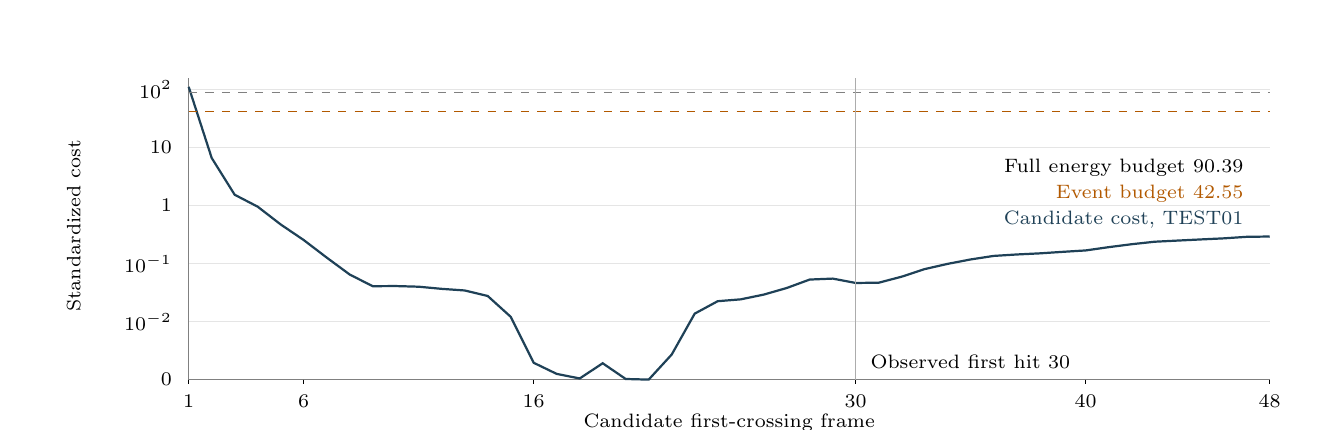
\begin{tikzpicture}[x=0.115in,y=0.29in,font=\scriptsize]
\clip (-6,-1.05) rectangle (49,5.4);
\draw[gray!20] (1,0.0) -- (48,0.0);
\node[anchor=east] at (0.7,0.0) {$0$};
\draw[gray!20] (1,1.0) -- (48,1.0);
\node[anchor=east] at (0.7,1.0) {$10^{-2}$};
\draw[gray!20] (1,2.0) -- (48,2.0);
\node[anchor=east] at (0.7,2.0) {$10^{-1}$};
\draw[gray!20] (1,3.0) -- (48,3.0);
\node[anchor=east] at (0.7,3.0) {$1$};
\draw[gray!20] (1,4.0) -- (48,4.0);
\node[anchor=east] at (0.7,4.0) {$10$};
\draw[gray!20] (1,5.0) -- (48,5.0);
\node[anchor=east] at (0.7,5.0) {$10^{2}$};
\draw[gray] (1,0) -- (48,0);
\draw[gray] (1,0) -- (1,5.2);
\draw[ink,line width=0.8pt] plot coordinates {(1,5.04853723) (2,3.82202089) (3,3.18732169) (4,2.98154928) (5,2.67508288) (6,2.40685821) (7,2.10414126) (8,1.81210826) (9,1.61053329) (10,1.61303539) (11,1.60171000) (12,1.56483420) (13,1.53708641) (14,1.44190405) (15,1.08315127) (16,0.28997916) (17,0.09850546) (18,0.01991584) (19,0.28178774) (20,0.01075546) (21,0.00000000) (22,0.43248402) (23,1.13765114) (24,1.35203878) (25,1.38385148) (26,1.46550886) (27,1.57948968) (28,1.72522844) (29,1.74152970) (30,1.66632736) (31,1.67078065) (32,1.77482412) (33,1.90554781) (34,1.99598851) (35,2.07202128) (36,2.13280410) (37,2.15744242) (38,2.17678700) (39,2.20285412) (40,2.22732305) (41,2.28379283) (42,2.33467630) (43,2.37735947) (44,2.39727753) (45,2.41679223) (46,2.43558544) (47,2.46208854) (48,2.46713450)};
\draw[gray,dashed] (1,4.95613472) -- (48,4.95613472);
\draw[orange!70!black,dashed] (1,4.62890072) -- (48,4.62890072);
\draw[gray!65,line width=0.3pt] (30,0) -- (30,5.2);
\node[anchor=west,fill=white,inner sep=1pt] at (30.5,.30) {Observed first hit 30};
\node[anchor=east,fill=white,inner sep=1pt] at (47,3.65) {Full energy budget 90.39};
\node[anchor=east,fill=white,inner sep=1pt,text=orange!70!black] at (47,3.20) {Event budget 42.55};
\node[anchor=east,fill=white,inner sep=1pt,text=ink] at (47,2.75) {Candidate cost, TEST01};
\draw (1,0) -- (1,-.07);
\node[anchor=north] at (1,-.10) {1};
\draw (6,0) -- (6,-.07);
\node[anchor=north] at (6,-.10) {6};
\draw (16,0) -- (16,-.07);
\node[anchor=north] at (16,-.10) {16};
\draw (30,0) -- (30,-.07);
\node[anchor=north] at (30,-.10) {30};
\draw (40,0) -- (40,-.07);
\node[anchor=north] at (40,-.10) {40};
\draw (48,0) -- (48,-.07);
\node[anchor=north] at (48,-.10) {48};
\node at (24.5,-.75) {Candidate first-crossing frame};
\node[rotate=90] at (-4,2.65) {Standardized cost};
\end{tikzpicture}
\end{center}

The event-score calibration threshold was $52.9\%$ smaller than the total-motion-energy calibration threshold. The former is not a certified bound on actual path energy. For TEST01, excluding frame 6 using the fixed event score would require a threshold below approximately $0.2552$, compared with $42.550$. Excluding all labels after the known prefix would require a threshold below approximately $0.2920$. The maximum comes from a CAL source with two censored labels. As a post-hoc sensitivity check, assigning censoring score zero would leave a finite-label calibration maximum of $32.109$, still above every retained known-prefix score (largest $6.638$).

\textbf{Calibration floor follow-up.} The archived floor analysis found all ten CAL run lower floors equal to zero; the largest outward upper bound on $|R-E|$ over their safe frames was $0.09816653879347023<0.20$. Under its numerical enclosure assumptions, the exact native threshold lies in the outer enclosure $[0,42.55011328277993]$. This computed enclosure is not asserted to be the exact attainable interval for the actual $R,E$: the exact upper endpoint is $q_{\rm upper}$, whereas the displayed value is an outward numerical bound $Q^+$. For the sole available 48-frame TEST prefix, frame 21 has candidate score upper bound zero and cannot be removed solely by lowering the calibration threshold. This is structural retention by the fixed score; the bound alone does not identify frame 21 as the first strict exceedance of $A_t$ or as the actual crossing. The other 66 labels of the public common set $\dates{6}{71}\cup\{\dd\}$ remain unresolved for the actual model by that analysis. For labels 49--71 and $\dd$, its check concerns the 48-frame prefix policy, not exact full-tail feasibility. The observed crossing is 30, the public common set remains 67 labels, and the other 11 TEST schedules lack generated prefixes. No narrower set is established. These results are recorded in the 6 November 2026 floor archive, \path{evidence/}\allowbreak\path{math4999_calibration_floor_20261106_001/}: \path{run02/result/RESULTS.json}, \path{ROOT_VERIFICATION.json}, and \path{VERIFIED.json}; their numerical claims retain the stated enclosure and provenance conditions.

Each full motion region covered 5 of 6 TEST source paths. The event surrogate was below its CAL maximum in 5 of 6 TEST sources as well, with a different excluded source. These are sufficient-condition checks. First-label coverage was 6 of 6 sources, including 11 schedules with universal fallback because their generated vectors are unavailable. That fallback is $\dates{1}{80}\cup\{\dd\}$, all 81 labels; it does not exclude frame 1 for those schedules. Direct TEST pixel-based evaluation concerns one of the 12 schedules. All 16 sources had been previously examined.




\subsection{Pixel-box calibration diagnostic}\label{sec:boxreplay}
A separately authorized local CPU diagnostic compared the radial surrogate, a safe-term box bound, and the two-sided box bound on the same five CAL sources and the one known TEST prefix. The arithmetic uses conditional norm enclosures and outward-rounded dual bounds described in the local implementation record. The thresholds are score upper bounds; decimals below are rounded for presentation, while decisions used exact fractions.
\begin{center}
\small
\begin{tabular}{lrrl}
\toprule
Calibration bound & Threshold & TEST labels & Finite hull \\
\midrule
Radial & 42.5501 & 80 & $2$--$80$ \\
Box, safe term & 33.8172 & 80 & $2$--$80$ \\
Box, two-sided & 33.8172 & 80 & $2$--$80$ \\
\bottomrule
\end{tabular}
\end{center}
Each TEST set is $\dates{2}{80}\cup\{\dd\}$ and contains the true label 30. The box threshold is about $20.52\%$ below the radial threshold, but neither the endpoint-narrowing primary criterion nor the secondary criterion of fewer than 67 total labels was met. No label of the public common set $\mathcal C_0=\dates{6}{71}\cup\{\dd\}$ was deleted. CAL01 schedule 0 is censored and determines both box maxima; the crossing-term refinement improves individual upper scores on the finite-crossing CAL runs but does not change the global maximum here.

All ten CAL box floor lower certificates remain zero. Under the stated numerical and provenance conditions the native threshold is contained in the outer enclosure $[0,33.818]$; this rounded outward interval is not an exact attainable or identified range. Only frame 21 is certified unavoidable by the floor comparison among the 67 common labels; the other 66 remain inconclusive under that check. The TEST labels were checked during preflight, but not used to choose thresholds or construct candidate scores; evaluation was summarized after sets were written. This was retrospective and not blinded. The 11 missing TEST schedules use universal fallback. Thus source-level both-schedule coverage was descriptively $6/6$, while the both-schedule primary success count was $0/6$; these counts do not establish independent generalization. Failure of this frozen variant does not establish that all pixel constraints are useless or that narrower sets are impossible for the model.

The single supervised attempt completed in 108.765 seconds; 11 fixed boundary tests passed within it, and the recorded peak working set and private commit were 499,134,464 and 1,293,979,648 bytes, respectively, both below the 1.5 GiB limit. It made no new model predictions, GPU rental, or downloads. The local records are in \path{evidence/}\allowbreak\path{math4999_box_execution_20261110_001/}\allowbreak\path{run001/}: \path{RESULTS.json}, \path{CANDIDATES.csv}, and \path{RECEIPT.json}. This retrospective calculation does not supply a new prospective coverage guarantee.

\section{Discussion and conclusion}\label{sec:discussion}
The deterministic results distinguish exclusion from attainment. In particular, the energy inversion is exact in its unrestricted product space, including the open crossing boundary, but a feasible abstract trajectory need not correspond to a pixel-feasible or physically realizable video. The scalar majorant is sharp for its specified information class; additional directional, pixel, or temporal information can change that class. The numerical claims depend on the stated floating-point and provenance assumptions, and the earlier directional diagnostic additionally depends on its norm and cosine enclosures.

The smaller event-score threshold did not translate into a useful narrowing of the individual set in this replay. The later zero-floor result leaves the effect of recovering native directions unresolved for the other 66 common labels, while certifying retention of frame 21 under threshold reduction alone. Direct test evaluation used one generated prefix, while the other 11 test schedules retained all 81 labels under universal fallback. The common-rule deletion is conditional on a separate transfer assumption. Prior examination of all sources and unavailable generated vectors preclude treating these retrospective results as prospective evidence of the conditional source-rank guarantee; that guarantee itself requires the stated exchangeability and a rule fixed before calibration and testing.

A two-sided pixel-box calibration and its conservative numerical design appear in Appendix~\ref{app:details}. The fixed diagnostic reduced the threshold but did not narrow the available individual set; this does not rule out gains from other pixel-aware methods. A next discriminating input would be native calibration forecast directions, allowing direct $C(T)$ calibration, together with an independently tested source-conditioned motion reference. Both require further validation before a narrower reliable individual range can be claimed.

Eight additional local source inputs have been prepared, with zero new model predictions; the original 16 sources remain retrospective. The frozen future validation design keeps the same checkpoint, $\tau$, two seed schedules and $H=80$, using the 48-frame prefix as primary and all 80 generated frames as secondary information. It would report source success only when both seeds contain their true labels, as $k/8$, along with full candidate counts and membership, censor inclusion, and failures or missing runs. The proposed refinement evaluates both seeds: each true label must be retained, the whole set must lie within $\mathcal C_0$, and its finite labels must either have an integer hull shorter than 66 frames or be absent with a correctly retained censoring label. Report censor-only outcomes separately, not as intervals. Finite hull endpoints and spans are null for an empty finite set; the 81-label fallback has finite hull 1--80. A smaller label count or holes alone do not establish a narrower time range. Report full membership, labels added or excluded, and fallback explicitly; coverage alone does not establish useful individual prediction. This is a proposal for separate authorization, not an executed experiment or a new $5/6$ batch guarantee; no iid confidence interval is claimed. See the 6 November 2026 expansion archive, \path{evidence/}\allowbreak\path{math4999_expansion_20261106_001/}: \path{READINESS_ZH.md}, \path{PROTOCOL.md}, and \path{VERIFIED.json}.

\newpage
\appendix
\section{Proof details and numerical conditions}\label{app:details}
\textbf{Source-level rank.} Conditional on DEV, let $J_1,\ldots,J_5,J_6$ be exchangeable source scores, including any maximum across the two schedules. Let $I_i$ indicate that $J_i$ is strictly larger than all five other scores. For every realization $\sum_{i=1}^6 I_i\le1$; exchangeability gives equal conditional expectations, so $\Pr(I_6=1\mid\mathrm{DEV})\le1/6$. Failure of $J_6\le\max_{i\le5}J_i$ is exactly $I_6=1$. This covers ties and lexicographic scores as well. Probability is marginal over CAL and the new source conditional on DEV, not conditional on the realized CAL set. No independence between schedules within a source is required. This supplies the rank step in Section~\ref{sec:calibration}, Proposition~\ref{prop:tube}, and Theorem~\ref{thm:event}.

\textbf{Projection and strict crossing in Theorem~\ref{thm:energy}.} Fix a frame and let $A=\norm{g-\mu}$. If $A>\tau$, the closest safe vector is $v=g+(\tau/A)(\mu-g)$; if $A\le\tau$, it is $v=\mu$. Thus the minimum safe cost is $(A-\tau)_+^2$, including $A=0$. For a crossing, if $A>\tau$ choose $v=\mu$, attaining zero cost. If $0<A\le\tau$, choose $v=g+(1+\delta)(\tau/A)(\mu-g)$ with $\delta>0$; its cost tends to $(\tau-A)^2$ but every crossing costs strictly more. If $A=0$, choose any unit vector $e$ and $v=g+(\tau+\delta)e$; the same conclusion holds. In particular $A=\tau$ has zero infimum but does not attain it. Independent frame choices attain all safe minima and can make the crossing cost arbitrarily close to its infimum. Hence, for $A_t\le\tau$, feasibility is exactly $C(t)<B$; for $A_t>\tau$, it is exactly $C(t)\le B$. This includes $B=0$. Censoring uses only attained safe minima and is feasible exactly when $C(\dd)\le B$. This unrestricted product-space result establishes exclusions under its assumptions; it does not establish attainment by a physical model or pixel-feasible video.

\textbf{Majorant and sharpness.} In Lemma~\ref{lem:majorant}, $E$ denotes the true norm, not its archived floating-point approximation. If $E\le\tau$, then $(R+E-\tau)_+\le R$, so the $R^2$ term in the safe minimum is redundant. If $E>\tau$, then $|R-E|\ge E-R>\tau-R$, hence $(\tau-|R-E|)_+\le R$, and the $R^2$ term in the crossing minimum is also redundant. For $R>0$, the two collinear constructions in Proposition~\ref{prop:sharp} attain the remaining terms. If $R=0$, choose any unit vector $e$ and $g=v+Ee$; then $A=E$, and the relevant contribution is zero. These choices preserve all exact errors and the first-crossing label. Numerical application to archived errors additionally requires valid enclosures of the exact norms; the mathematical inequalities alone do not establish those enclosures.

\subsection*{A pixel-aware upper bound for future study}
\begin{lemma}[Box-constrained ball support]\label{lem:box}
For a frame let $w=v-\mu$, $e=g-v$, $R=\norm w$, and $E=\norm e$, using the RMS inner product above. If the true and generated frames lie in $[0,1]^D$, then $-x\le e\le1-x$ coordinatewise. Define
\[
 M_E(w,x)=\max_{\substack{-x\le z\le1-x\\\norm z\le E}}\ip{w}{z}.
\]
Then $A^2\le R^2+E^2+2M_E(w,x)$ and $M_E\le RE$. For a safe frame, the first term in Lemma~\ref{lem:majorant} remains $R^2$ and its other upper-bound term may use $\sqrt{R^2+E^2+2M_E}$ in place of $R+E$. The crossing term is unchanged.
\end{lemma}
\begin{proof}
The actual error $e$ is feasible, and expanding $\norm{w+e}^2$ proves the first inequality; Cauchy--Schwarz gives the second. To compute $M_E$, let $z_i^*=1-x_i$ if $w_i>0$, $z_i^*=-x_i$ if $w_i<0$, and $z_i^*=0$ otherwise, and put $r^*=\norm{z^*}$. If $E=0$ the maximum is zero; if $E\ge r^*$, $z^*$ attains the unrestricted box support. For $0<E<r^*$, the continuous function $\norm{\operatorname{clip}(\lambda w,-x,1-x)}$ goes from zero to $r^*$, so some finite $\lambda>0$ makes it equal $E$. The clipped vector maximizes $\ip{w}{z}-\norm z^2/(2\lambda)$ coordinatewise over the box. For any feasible $z$, its norm is at most $E$, so this maximizing property proves its support value is at least $\ip{w}{z}$. This also covers zero coordinates, boundary pixels, and saturation.
\end{proof}
The ball relaxation bounds the fixed-error sphere and need not attain its exact extremum. A proposed two-sided extension uses $M_+=M_E(w,x)$ and $M_-=M_E(-w,x)$ and sets
\begin{align*}
 a_-^2&=\max\{(R-E)^2,0,R^2+E^2-2M_-\},\\
 a_+^2&=\min\{(R+E)^2,R^2+E^2+2M_+\}.
\end{align*}
Expanding $\norm{w+e}^2$ and using the feasibility of $e$ gives $a_-\le A\le a_+$. Thus the safe upper contribution is $\min\{R^2,(a_+-\tau)_+^2\}/\sigma^2$ and the crossing upper contribution is $\min\{R^2,(\tau-a_-)_+^2\}/\sigma^2$. Summing as in $\overline C$ gives $C(T)\le\overline C_{\rm two}\le\overline C_{\rm safe}\le\overline C_{\rm radial}$. Maximizing over the same CAL runs and thresholding the same candidate score gives nested sets in the same order. These are nested score thresholds, not an intersection of separately calibrated candidate scores. Under the fixed-rule and conditional source-exchangeability assumptions, the source-rank proof remains applicable; reuse of the old CAL sources does not establish a fresh empirical guarantee.

Similarly, define $L_{\rm box}(T)$ by summing $(a_--\tau)_+^2/\sigma^2$ on safe frames and, for a finite crossing, $(\tau-a_+)_+^2/\sigma^2$ at that frame. Censoring sums all $H$ safe terms. Then $L\le L_{\rm box}\le C(T)$ and, taking the CAL maximum,
\[
 q_{\rm floor}\le q_{\rm floor,box}\le q_{\rm native}
 \le Q_{\rm box}\le Q_{\rm radial}.
\]
A candidate upper score no larger than a certified lower bound on $q_{\rm floor,box}$ cannot be removed by recovering CAL directions alone under the fixed prefix policy; failure of that comparison is inconclusive. A floor is not a replacement calibration threshold. These box bounds are not asserted sharp or attainable; the exact interval result in Proposition~\ref{prop:floor} remains restricted to its unrestricted geometry.

For an operational upper bound on $M_E(w,x)$, any $\lambda\ge0$ gives
\[
 B_\lambda(w)=\lambda E^2+D^{-1}\!\sum_i
 \max_{-x_i\le z\le1-x_i}(w_i z-\lambda z^2)\ge M_E(w,x).
\]
For $\lambda>0$ the maximizer is the coordinatewise clip of $w_i/(2\lambda)$ to the box; at zero use a favorable endpoint. Feasibility and $\norm z\le E$ prove the inequality. For $R,E>0$, completing the square at the exact $\lambda=R/(2E)$ and writing $\delta_\pm=\operatorname{dist}(\pm Ew/R,K)$ gives
\[
 (R-E)^2+(R/E)\delta_-^2\le A^2
 \le(R+E)^2-(R/E)\delta_+^2.
\]
Here distance uses the RMS norm; if $R=0$ then $A=E$, and if $E=0$ then $A=R$. A stored approximate ratio instead requires the general dual expression with certified outward bounds. Because distance is subtracted, its lower bound is needed to certify an upper bound. Any chosen dual parameters give valid bounds, but an approximate primal value is not an upper bound.

The mathematical bounds do not guarantee empirical improvement. The accompanying \path{BOX_CALIBRATION_THEORY.md} and \path{EXPERIMENT_DESIGN_20261110.md} specify the fixed two-parameter numerical scheme and enclosure conditions. Section~\ref{sec:boxreplay} reports the separately authorized diagnostic; it did not produce a narrower prediction set.

\textbf{Prefix containment.} For $t\le K$ the prefix score equals the full score. For $t>K$ the full score includes all nonnegative terms in $C_K^{\rm tail}$, as does the full censoring score. Consequently $C_K^{\rm tail}\le C(t)$ and $C_K^{\rm tail}\le C(\dd)$, so thresholding the lower scores retains every label retained by the exact full-score set.

\subsection*{Numerical conditions and their consequences}
\textbf{Conditional binary64 norm enclosure.} Let $D=196608$, $u=2^{-53}$, $\lambda=2^{-1074}$ and $\gamma_n=nu/(1-nu)$. Suppose stored coordinates $a,b\in[0,1]$, $c\in[-2,2]$, and define exact $z=a-b-c$. Compute $\widehat z=\operatorname{fl}(\operatorname{fl}(a-b)-c)$, square each coordinate, sum each nonnegative term exactly once using at most $D-1$ additions in any tree, divide by $D$, and take a square root. Assume binary64 round-to-nearest, gradual underflow, no overflow, and $|\operatorname{fl}(q)-q|\le u|q|+\lambda$ for each elementary operation including square root. The floating-point error model and $\gamma_n$ notation follow \cite[Chapters 2--4]{higham2002}; the explicit RMS bound below is derived for this report. These platform and provenance assumptions are not machine-verified here.

The two subtractions give $|\widehat z-z|\le5u+4\lambda$ coordinatewise and $|\widehat z|<4$. The RMS triangle inequality gives $|\norm{\widehat z}-\norm z|\le\norm{\widehat z-z}\le5u+4\lambda$. Put $m=D^{-1}\sum_j\widehat z_j^2$ and let $\widehat m$ be the computed mean square before the square root. The standard product bound for at most $D+1$ relative operations along each term, together with $D$ squaring and at most $D-1$ additive underflow errors divided by $D$, yields $|\widehat m-m|\le\gamma_{D+8}m+8\lambda$. For nonnegative $x,m$, if $0\le\gamma<1$, $\epsilon\ge0$, and $|x-m|\le\gamma m+\epsilon$, then $|\sqrt{x}-\sqrt m|\le\gamma\sqrt m+\sqrt\epsilon$. Applying this and the square-root rounding bound, and using $\sqrt m<4$, gives
\[
 |\widehat r-r|\le4\gamma_{D+8}+10u+5\lambda+\sqrt{8\lambda}<10^{-9},
\]
where $r$ is the exact RMS of $z$. Endpoint rounding of $\operatorname{fl}(\widehat r\pm\text{stored }10^{-7})$ contributes less than $10^{-15}$, while the stored guard exceeds $0.99\cdot10^{-7}$. Thus the guarded interval contains $r$, including at zero and for tiny norms. This applies to the archived float64 error with $c=0$ only when its computation has the stated provenance, and to residuals using the frozen stored $\mu$; later comparisons use exact fractions. It does not certify the older direction or cosine pipeline, whose conclusions remain conditional on their stated enclosures.


\subsection*{Conservative score evaluation}
\textbf{Enclosure formulas.} For exact norms $R,E,A$, suppose $R\in[R^-,R^+]$, $E\in[E^-,E^+]$, and $A\in[A^-,A^+]$, with nonnegative endpoints. Define
\[
 d_{RE}=\max\{0,R^- - E^+,E^- - R^+\}
       =\min_{r\in[R^-,R^+],\ e\in[E^-,E^+]}|r-e|.
\]
With each scale $\sigma_t$ treated as its fixed, stored, exact positive value, upper bounds for the safe and crossing contributions are
\begin{align*}
 u_{t,\mathrm{safe}}^+&=\frac{\min\{(R_t^+)^2,(R_t^++E_t^+-\tau)_+^2\}}{\sigma_t^2},\\
 u_{t,\mathrm{cross}}^+&=\frac{\min\{(R_t^+)^2,(\tau-d_{R_tE_t})_+^2\}}{\sigma_t^2}.
\end{align*}
Each argument of each minimum is an upper bound for the corresponding true contribution, so their minimum is also an upper bound. It is not asserted to be the exact joint maximum of the minimum over the rectangle. For a finite candidate $t$, a lower score is
\[
 C^-(t)=\sum_{s<t}\frac{(A_s^- -\tau)_+^2}{\sigma_s^2}
       +\frac{(\tau-A_t^+)_+^2}{\sigma_t^2}.
\]
The prefix tail lower score is $p=\sum_{s\le K}(A_s^- -\tau)_+^2/\sigma_s^2$. For every $t>K$, $C(t)\ge C_K^{\rm tail}\ge p$, and $C(\dd)\ge C_K^{\rm tail}\ge p$; hence an ideally accepted tail label is retained whenever $p\le Q^+$. These inequalities follow from monotonicity of the positive-part terms and remain valid with exact rational arithmetic on the stored endpoints.

\textbf{From enclosures to the implemented set.}
Write $\underline C_a(y)$ for the computed lower candidate score and $\overline J_i^{\,+}$ for the computed upper source surrogate. Valid norm enclosures and exact rational score arithmetic give
\[
 \underline C_a(y)\le C_a(y),\qquad
 Q^+=\max_{i\in{\rm CAL}}\overline J_i^{\,+}
       \ge\max_{i\in{\rm CAL}}J_i=Q.
\]
Hence $C_a(y)\le Q$ implies $\underline C_a(y)\le Q^+$. The implemented conservative set contains the ideal score set, including equality and the unknown-tail fallback. Thus numerical conservatism cannot remove an ideally accepted true label when the enclosure assumptions hold. For every archived DEV, CAL and TEST error, the code requires $E_t^+<\tau$ or $E_t^->\tau$ before assigning its exact label; it aborts if an interval meets the threshold. This criterion applies to the error $E_t$, not the generated displacement $A_t$. The observed separation exceeds $10^{-7}$ in this replay. This does not verify exchangeability, erase prior reuse of the sources, or certify the omitted directional pipeline.


\begin{thebibliography}{9}
\bibitem{vovk2005}
V. Vovk, A. Gammerman and G. Shafer.
\emph{Algorithmic Learning in a Random World}.
Springer, New York, first edition, 2005.
\href{https://doi.org/10.1007/b106715}{doi:10.1007/b106715}.

\bibitem{diquigiovanni2021}
J. Diquigiovanni, M. Fontana and S. Vantini.
\emph{Conformal Prediction Bands for Multivariate Functional Data}.
arXiv:2106.01792v1, 2021.
\url{https://arxiv.org/abs/2106.01792v1}.

\bibitem{higham2002}
N. J. Higham.
\emph{Accuracy and Stability of Numerical Algorithms}.
Society for Industrial and Applied Mathematics, Philadelphia,
second edition, 2002.
\href{https://doi.org/10.1137/1.9780898718027}{doi:10.1137/1.9780898718027}.
\bibitem{kassis2026}
T. Kassis, V. Agarwal, Y. He, D. Patel and A. M. Brueckner.
\emph{Scientific Agent Skills: A Library of Procedural Knowledge for Research Agents}.
arXiv:2609.00065, 2026.
\href{https://doi.org/10.48550/arXiv.2609.00065}{doi:10.48550/arXiv.2609.00065}.
\end{thebibliography}

\textbf{Scope of attribution.}
The first three references supply the conformal-prediction background and standard rounding-error framework. The scientific-writing skill associated with \cite{kassis2026} assisted the organization and revision of this draft; it is not evidence for the mathematical or empirical claims. The first-crossing inversion, residual/error-length majorant, its stated geometric sharpness, and the specialized numerical bounds are proved explicitly in this report. The finite-data observations come from the archived local study; the references do not establish prospective validity for those reused videos.

\end{document}
